\documentclass[a4paper,12pt]{article}

%%% Работа с русским языком
\usepackage{cmap}					% поиск в PDF
\usepackage{mathtext} 				% русские буквы в фомулах
\usepackage[T2A]{fontenc}			% кодировка
\usepackage[utf8]{inputenc}			% кодировка исходного текста
\usepackage[english,russian]{babel}	% локализация и переносы

%%% Дополнительная работа с математикой
\usepackage{amsfonts,amssymb,amsthm,mathtools} % AMS
\usepackage{amsmath}
\usepackage{icomma} % "Умная" запятая: $0,2$ --- число, $0, 2$ --- перечисление

%% Номера формул
%\mathtoolsset{showonlyrefs=true} % Показывать номера только у тех формул, на которые есть \eqref{} в тексте.

%% Шрифты
\usepackage{euscript}	 % Шрифт Евклид
\usepackage{mathrsfs} % Красивый матшрифт

%% Свои команды
\DeclareMathOperator{\sgn}{\mathop{sgn}}

%% Перенос знаков в формулах (по Львовскому)
\newcommand*{\hm}[1]{#1\nobreak\discretionary{}
{\hbox{$\mathsurround=0pt #1$}}{}}

%%% Работа с картинками
\usepackage{graphicx}  % Для вставки рисунков
\graphicspath{{images/}{images2/}}  % папки с картинками
\setlength\fboxsep{3pt} % Отступ рамки \fbox{} от рисунка
\setlength\fboxrule{1pt} % Толщина линий рамки \fbox{}
\usepackage{wrapfig} % Обтекание рисунков и таблиц текстом

%%% Работа с таблицами
\usepackage{array,tabularx,tabulary,booktabs} % Дополнительная работа с таблицами
\usepackage{longtable}  % Длинные таблицы
\usepackage{multirow} % Слияние строк в таблице

\usepackage[english,russian]{babel}
\usepackage{indentfirst}
\usepackage{misccorr}
\usepackage{graphicx}
\usepackage{amsmath}

%%% Заголовок
\usepackage[utf8]{inputenc}

\title{Week2(Task)}
\author{pyatkovsky15022001 }
\date{September 2020}

\begin{document}

\maketitle

\section{}

2. Пусть рис.\ref{tab:main_mean} представляет положения Солнца S, Земли T
и Луны L, и пусть тэта есть центр тяжести Земли и Луны. Делаем следующие обозначения:

\begin{table}[!h]
    \begin{center}
        \caption{Обозначения}\label{tab:main_mean} 
        \begin{tabular}{|r|c|}
            \hline Масса Солнца & S \\ \hline
            \dots Земли & T\\ \hline
            \dots Луны & L\\ \hline
        \end{tabular}
    \end{center}
\end{table}


Расстояние:
\begin{equation*}
    S \times \Theta = \rho;\;
    S \times T = \rho1;\;
    S \times L = \rho2;\;
    T \times L = r;\;
\end{equation*}
Тогда будет:
\begin{equation}
    \begin{aligned}
        &T \Theta = r1 = \frac{L}{T +L} \cdot r\\
        &L \Theta = r2 = \frac{T}{T +L} r
    \end{aligned}
\end{equation}

Составим теперь выражения ускорений,которые эти тела сообщают друг другу.

\begin{figure}[bhtp]
    \centering
    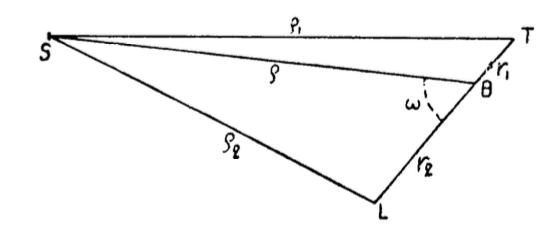
\includegraphics{21.png}
    \caption{}
    \label{fig:21}
\end{figure}

Солнце S сообщает ускорения:
\begin{center}
    Земле: \; $f\cdot \frac{S}{\rho_{1}^2}$ \;по\;направлению\; TS \\
    Луне: \; $f\cdot \frac{S}{\rho_{2}^2}$ \; >> \;\;\; >> \;\;\;LS\\
\end{center}
вследствие чего точка $\Theta$ \:имеет\:ускорения:

\begin{center}
    $\frac{T}{T+L} \cdot f \cdot \frac{S}{\rho_{1}^2}$\;по\; направлению,\,параллельному\;$TS$\\
    $\frac{L}{T+L} \cdot f \cdot \frac{S}{\rho_{2}^2}$ \: >> \;\;\; >> \;\; $LS$ \\
\end{center}

Ускорения Солнца, происхожящие от притяжения Земли и Луны, соответсвенно, суть:
\begin{center}
    $f \cdot \frac{T}{\rho_{1}^2}$ по направлению $ST$\\
    $f \cdot \frac{L}{\rho_{1}^2}$ по направлению $SL$\\
\end{center}
поэтому ускорения точки $\Theta$ относительно точки $S$ будут:
\begin{center}
    $w_1 = f\cdot \frac{\left(S+T+L\right)}{T+L} \cdot \frac{T}{\rho_{1}^2}$ по направлению параллельно $TS$ \\
    $w_2 = f\cdot \frac{S+T+L}{T+L} \cdot \frac{L}{\rho_{2}^2}$ по направлению параллельно $LS$ \\
\end{center}
Разлагая эти ускорения,соответсвенно,по направлениям, $\Theta S$ и $\Theta L$, получим,как легко видеть из подобия показанныех на рис.\ref{fig:22} и рис.\ref{fig:23} треугольников:
\begin{equation*}
    \begin{aligned}
        \acute{w_1} = w_1 \cdot \frac{\rho}{\rho_1} \:по\:напралению\: \Theta S \\
        \acute{\acute{w_1}} = w_1 \cdot \frac{r_1}{\rho_1} \;>>\;\;\; >>\;\; \Theta L \\
        \acute{w_2} = w_2 \cdot \frac{\rho}{\rho_2} \;>>\;\;\; >>\;\; \Theta S \\
        \acute{\acute{w_2}} = w_2 \cdot \frac{r2}{\rho_2} \;>>\;\;\; >>\;\; L\Theta  \\
    \end{aligned}
\end{equation*}

\begin{figure}[h!]
    \centering
    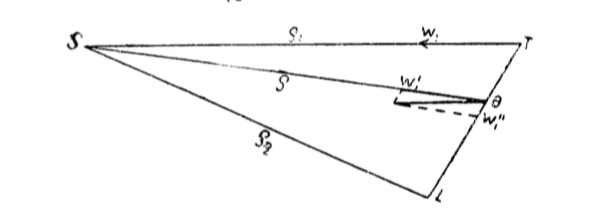
\includegraphics{22.png}
    \caption{}
    \label{fig:22}
\end{figure}
получим для ускорений точки $\Theta$ слагающие:
\begin{equation*}
    \begin{aligned}
        W_1 = \acute{w_1} + \acute{w_2} = f\cdot\frac{S + T + L}{T + L}\cdot \left[T\cdot \frac{\rho}{\rho_{1}^3} + L\cdot\frac{\rho}{\rho_{2}^3}\right] по\:\Theta S\\
        W_2 = \acute{\acute{w_1}} - \acute{\acute{w_2}} = f\cdot\frac{S + T + L}{T + L}\cdot \left[T\cdot \frac{\rho_1}{\rho_{1}^3} - L\cdot\frac{\rho}{\rho_{2}^3}\right] по\: \Theta L\\
    \end{aligned}
\end{equation*}

\begin{wrapfigure}{l}{0.3\linewidth}
    \centering
    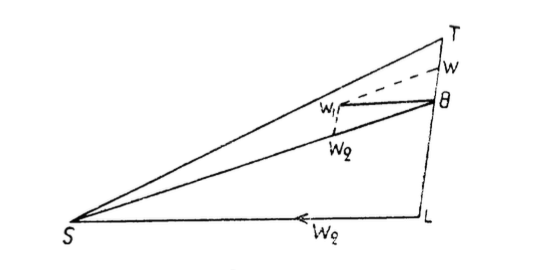
\includegraphics[scale = 0.5]{23.png}
    \caption{}
    \label{fig:23}
\end{wrapfigure}


Заменив $\rho_1$ и $\rho_2$ и выражениями (1), имеем:
\begin{center}
    \begin{equation*}
        \begin{aligned}
            W_1 = f\cdot\frac{S + T + L}{T + L}\cdot{\rho}\cdot\left[\frac{T}{\rho_{1}^3} + \frac{L}{\rho{_2}^3} \right] по направлению\: \Theta S \\
             W_1 = f\cdot\frac{S + T + L}{(T + L)^2}\cdot T \cdot L \cdot r \cdot\left[\frac{1}{\rho_{1}^3} - \frac{1}{\rho{_2}^3} \right] по направлению\: \Theta S \\
        \end{aligned}
    \end{equation*}
\end{center}
Но
\begin{equation*}
    \begin{aligned}
        \rho_1^2 = \rho^2 + 2\rho\cdot\frac{L}{T + L}\cdot r \cos w + \left(\frac{L}{T + L}\cdot r\right)^2 \\
        \rho_2^2 = \rho^2 - 2\rho\cdot\frac{L}{T + L}\cdot r \cos w + \left(\frac{L}{T + L}\cdot r\right)^2 \\
    \end{aligned}
\end{equation*}
следовательно:
\begin{equation*}
    \begin{aligned}
    \frac{1}{\rho_1^3} = \frac{1}{\rho^3}\left[1\:+\:3\frac{L}{T + L}\cos w +\left(\frac{L}{T + L}r\right)^2\left(-\frac{3}{2}+\frac{15}{2}\cos^2 w\right)+\cdots\right]\\
    \frac{1}{\rho_2^3} = \frac{1}{\rho^3}\left[1\:+\:3\frac{L}{T + L}\cos w +\left(\frac{L}{T + L}r\right)^2\left(-\frac{3}{2}+\frac{15}{2}\cos^2 w\right)+\cdots\right]\\
    \end{aligned}
\end{equation*}
Подставляя эти выражения, имеем:
\begin{equation*}
    \begin{aligned}
        W_1 = f\cdot\frac{S + T + L}{\rho^2}\left[1\:+\:\frac{T\cdot L}{(T + L)^2}\cdot\frac{r^2}{\rho^2}\left(-\frac{3}{2}+\frac{15}{2}\cos^2 w\right)+\cdots\right]\\
         W_2 = f\cdot\frac{S + T + L}{\rho^2}\left[-3\cdot\frac{T\cdot L}{(T + L)^2}\cdot\frac{r^2}{\rho^2}\left(-\frac{3}{2}+\frac{15}{2}\cos^2 w\right)+\cdots\right]\\
    \end{aligned}
\end{equation*}
Но отношения:
\begin{equation*}
    \frac{L}{T+L}\approx\frac{1}{80};\;\;\frac{r}{\rho}\approx\frac{1}{400};\;\;\left(\frac{r}{\rho}\right)^2 = \frac{1}{160000}\\
\end{equation*}
поэтому будет
\begin{equation*}
    \frac{T\cdot L}{(T + L)^2}\cdot\frac{r^2}{\rho^2} \approx \frac{1}{12800000}
\end{equation*}
и члены, содержащие этот множитель, могут быть отброшены, так что будет:
\begin{equation*}
    \begin{aligned}
        W_1 = f\cdot\frac{S + T + L}{\xi} по направлению \Theta S\\
        W_2 = 0 по направлению \Theta L
    \end{aligned}
\end{equation*}

Отсюда следует,что точка $\Theta$ движется вокруг Солнца по эллиптической орбите по законам Кеплера.

Рассмотрим теперь ускорение Луны по отношению к Земле, для чего к учкорениям, сообщаемым Луне Солнцем и Землею, надо присовокупить ускорение, равное и противоположное ускореию Земли, происходящему от действия Солнца и Луны. Поступив подобно предыдущему,получим:
\begin{equation*}
    \begin{aligned}
        f\cdot\frac{T + L}{r^2} + f\cdot S\left[\frac{r_2}{\rho_2^3} + \frac{r_1}{\rho_1^3}\right] по направлению L\Theta \\
        f\cdot\S\cdot\rho\left[\frac{1}{\rho_2^3} - \frac{1}{\rho_1^3}\right] по направлению \Theta S \\
    \end{aligned}
\end{equation*}
положим:
\begin{equation}
    T + L = \mu;\:S = M 
\end{equation}


\listoffigures

\listoftables


\end{document}
